% Chapter 4

\chapter{基于注意力机制的跨分辨率遥感影像计数}
在本节中,将详细介绍一种全新的基于注意力机制的跨分辨率遥感影像计数方法。通过分析CRVC数据集中数据的时间连续性和空间一致性特性,在现有网络基础上,设计了跨分辨率空间注意力和低分辨率下的时空注意力模块,充分结合了图像中的不同尺度,位置信息。
\section{问题分析}
由于直接从极低分辨率的图像中识别出车辆目标具有相当大的难度,本文通过将车辆计数问题转化为图像分割和回归问题来解决这一挑战。这种转换使得处理变得更为可行,是因为不论图像分辨率如何变化,同一类别的车辆数量与车辆实际占用面积之间的线性关系是恒定的。通过数据集中高分辨率图像的计数结果作为同一天同一地点的低分辨率图像的真值是有效的,同时解决了无法直接在低分辨率图像上人工计数得到真值的问题。车辆面积的计算需要基于车辆覆盖率(在图像中的车辆区域百分比)。为了计算车辆覆盖率,我们首先需要通过图像分割技术准确地从低分辨率图像中提取出车辆区域。因此,本文提出的车辆计数大致流程如下:
\begin{enumerate}    
\item 跨分辨率图像处理:我们将选择性地输入高分辨率图像以及与该高分辨率图像同一天的低分辨率图像,同时还包括距离该日期较近和较远的两张低分辨率图像。这些图像被输入到我们精心设计的分割网络中,该网络专门针对从极低分辨率图像中有效分割车辆区域进行了优化。
\item 车辆覆盖率的计算:通过应用先进的图像处理算法,网络将输出车辆的分割图。这些分割图将用于计算每个车辆的覆盖率,即每辆车在图像中所占的面积与整个图像面积的比例。
\item 车辆面积的转换与回归分析:将得到的车辆覆盖率转换为实际车辆面积,这一步是通过与车辆实际占用面积和数量之间的已知线性关系相结合完成的。我们将使用从高分辨率图像中得到的数据来计算回归模型的系数,这些系数反映了车辆面积与车辆数量之间的关系。然后,这些回归模型系数被应用到低分辨率图像上,以估计出车辆的数量。
\end{enumerate}
通过上述流程处理,即使这些低分辨率图像在视觉上难以分辨车辆细节,我们也能够参照高分辨率图像在极低分辨率图像中有效地进行车辆计数。此方法不仅提高了车辆计数的准确性,还为处理其他低分辨率图像分析任务提供了可能的方法论指导。
\section{网络设计}
网络设计如图8所示,网络基于CRVC-Net骨干网络搭建,采用U-Net编码器解码器结构。对于目标低分辨率图像,通过多层卷积网络组成的编码器提取出特征,用作后续解码器输入的一部分。在该编码器结构中,同时保留各层的中间结果,以便后续解码器中对应层使用。

为了利用来自高分辨率图像的先验空间信息和来自其他低分辨率图像的时间连续性约束,引入了两个监督分支跨分辨率空间一致性分支CRSC(crossresolution spatial consistency) 和同分辨率下时间一致性分支IRTC(intraresolution time continuity)。CRSC分支采用和主干编码器相同的架构,提取来自相应高分辨率图像的特征,以使同一天高分辨率图像和低分辨率图像的提取特征尽可能相似。IRTC分支共享主分支的模型及参数,提取来自距离该日期较近和较远的两张低分辨率图像的特征,后续将比较他们和主分支输出的差异。这是因为编码器应具有提取同一分辨率下所有图像的能力,而对于不同分辨率图像来说,像素密度不同导致图像细节不同,采取独立训练的编码器能更好表征不同细节特征,避免造成高分辨率图像细节的丢失,从而影响其指导能力。解码器接受主分支特征作为输入,同时在每一层解码器处,使用对应层的主分支及近处和远处低分辨率图像和高分辨率图像的中间结果作为key,设计了专门的注意力门,综合多渠道输入,进行解码。逐层操作直至生成分割图像。
\section{编码器}

\section{多来源注意力机制}
注意力机制有助于掌握时序信息,同时对于综合不同特征间相关关系有着很强的综合能力。本文中就针对CRVC数据集的特点,设计了自注意力门 SAG(Self Attention Gate)、跨分辨率注意力门 CAG(Crossresolution Attention Gate)和时间序列注意力门 TAG(Timeseires Attention Gate)三种注意力门模块,来充分利用数据集中的时间一致性和空间连续性特征。

如第二章所述,注意力机制主要需要三个输出,分别为key,query和value,通过下述公式可计算得出:
\begin{equation}
\text{Attention}(Q, K, V) = \text{Softmax}\left(\frac{QK^T}{\sqrt{d_k}}\right)V 
\end{equation}

首先是自注意力门,用主分支编码器对应中间层的结果作为key,解码器上一层上采样结果作为query和value进行计算。
跨分辨率注意力门,用CRSC分支编码器对应中间层的结果作为key,解码器上一层上采样结果作为query和value进行计算。
时间序列注意力门,用两个IRTC编码器对应中间层的结果分别作为key,解码器上一层上采样结果作为query和value进行计算。
\begin{figure}[h]
    \centering
    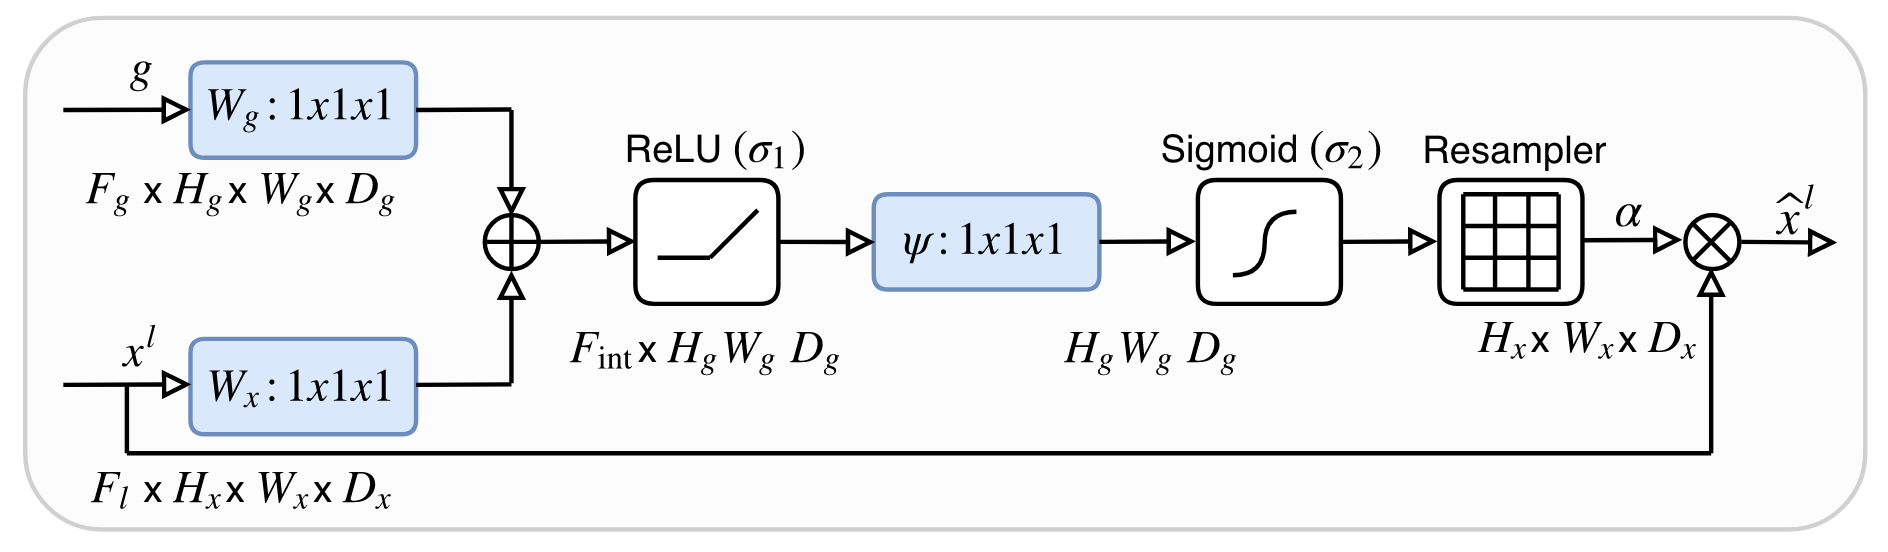
\includegraphics[width=\textwidth]{attentionG.png}
    \caption{U-Net网络结构}
    \label{fig:UNet}
  \end{figure}
本设计使用主分支、CRSC分支和IRTC分支分别作为key对解码器上一层上采样后的输出进行注意力操作。这种设计可以更精细地控制不同分支对最终输出的贡献,从而提升模型的性能和泛化性。

具体步骤如下
\begin{enumerate}    
    \item 获取Key和Query:Key来自于主分支、CRSC分支和IRTC分支的特征图。 Query则来自于解码器上一层的输出。
    \item 计算注意力权重: 使用query与每个key进行点积(或其他相似度计算方法),然后应用softmax函数来获取注意力权重。
    \item 应用注意力权重:使用得到的注意力权重对各分支的特征图进行加权求和,生成加权的特征图。
    \item 融合和上采样:将加权的特征图输入到解码器的当前层,进行上采样和进一步的处理。
\end{enumerate}

本文设计的网络将主分支、CRSC分支和IRTC分支编码器的对应层的中间结果分别用作注意力机制中的key,而对应的query和value则均来自上一层解码器的输出。这种设计允许模型在每一步解码过程中都重新评估各个编码器分支的重要性,更加动态地融合信息。此方法允许模型根据解码器的当前状态动态调整各个分支的权重,在反向传播中加以修改优化。同时通过考虑来自不同时间和空间信息的多个分支,模型能够更全面的利用数据集中的全部信息。

\section{解码器}

\section{损失函数}
与CRVC-Net类似,本设计中也包含其中的三个损失函数,不同的是本设计中额外使用焦点损失(Focal Loss)作为交叉熵函数的补充。

对于高分辨率和低分辨率图像间的空间一致性,使用下面的损失函数进行约束。
\begin{equation}
    \mathcal{L}_{\text {dif }}=\sum_{i}\left|F_l^{L R}-F^{HR}_{l}\right|^2
\end{equation}

对于时间连续性的约束,日期接近的图像间的差异应该小于日期相隔较远的差异。使用下面的损失函数进行约束。
\begin{equation}
    \mathcal{L}_{\text {ser }}=\sum_{l=1}^{m} \frac{\left|F_{\text {closel }}^{L R}-F^{L R}{ }_{l}\right|}{\left|F_{\text {far } l}^{L R}-F^{L R}_ l\right|}
\end{equation}

\subsection{焦点损失函数}
焦点损失函数(Focal Loss)最初是为解决目标检测中的类别不平衡问题设计的,尤其是在目标识别中背景与前景类别之间的不平衡问题。然而,这种损失函数的设计原理使其同样适用于广泛的多分类问题,特别是在存在明显类别不平衡的情况下。对于包含多种车辆类型的CRVC数据集,各类车辆数量极不平衡,其中包括轿车35844辆、小型货车737辆、大型货车1211辆、起重机60辆。 如果数据集中某些类型的车辆比其他类型少得多,使用焦点损失函数可以带来明显的优势。由于轿车数量显著多于其他几类车辆,采用交叉熵函数时
\begin{equation}
    \mathcal{L}_{\text {ent }}=-\frac{1}{n} \sum_{i} y_{i} \ln a_{i}
\end{equation}
其中的轿车样本占大多数,将显著影响损失函数整体的值,而缩小其他类别对于损失函数的贡献。因此在最终得到的网络中,对于其他几类的分类效果也因此受到影响。


焦点损失函数是交叉熵损失函数的一种改进。焦点损失函数通过重新设计交叉熵损失,可以调节不同数量样本之间的权重,从而使模型对于少量样本的表示能力更强,从而提高模型整体性能。


焦点损失函数的定义如下:
\begin{equation}
    FL(p_t) = -\alpha_t (1 - p_t)^\gamma \log(p_t)
\end{equation}

其中:\( p_t \) 是模型对当前样本的预测概率,对于正样本 \( p_t = p \),对于负样本 \( p_t = 1 - p \)。 \( \alpha_t \) 是平衡正负样本权重的系数,通常设置为一个小于 1 的值,用来增加少数类的重要性。\( \gamma \) 是调整易分类样本对损失的影响的聚焦参数,\( \gamma \geq 0 \)。当 \( \gamma = 0 \) 时,Focal Loss 退化为标准的交叉熵损失。\( \gamma \) 的值越大,对易分类样本的惩罚就越大。


通过引入调制因子 \( (1 - p_t)^\gamma \):当一个样本被错误分类,并且错误程度很大(即 \( p_t \) 很小)时,\( (1 - p_t)^\gamma \) 接近 1,损失不受影响。当一个样本被正确分类,且分类器置信度很大时(即 \( p_t \) 很大)时,\( (1 - p_t)^\gamma \) 接近 0,这使得这类样本对总损失的贡献大大降低,这样可以让模型集中精力学习那些难以分类的样本。


在多分类问题中,焦点损失函数的应用类似于其在二分类中的用法,但需要一些调整来处理多个类别。多分类版本的焦点损失函数通常表示为:

\begin{equation}
    FL(p_t) = - \sum_{c=1}^C \alpha_c (1 - p_{t,c})^\gamma \log(p_{t,c})
\end{equation}


其中:
\( C \) 是类别的总数。\( p_{t,c} \) 是模型对于每个类别 \( c \) 的预测概率。如果样本属于类别 \( c \),则 \( p_{t,c} \) 是该类别的预测概率;否则为 \( 1 - p_{t,c} \)。\( \alpha_c \) 是针对类别 \( c \) 的平衡系数,用于调节不同类别间的不平衡。\( \gamma \) 是聚焦参数,用来减小易分类样本的损失贡献,增加难分类样本的影响。


通过调节 \( \alpha_c \) 和 \( \gamma \) 参数,焦点损失函数可以帮助模型更好地学习那些样本数量较少的类别。这是通过增加这些类别样本的损失贡献来实现的,从而使模型在训练过程中更加关注它们。通过 \( (1 - p_{t,c})^\gamma \) 这一调节项,焦点损失函数提高了那些模型难以正确分类的样本的损失权重,从而激励模型改进这些区域的预测性能。


对于一个批次中的所有样本,焦点损失函数完整的表达式通常写作:

\begin{equation}
    \mathcal{L}_{\text {FL}} = -\frac{1}{N} \sum_{i=1}^{N}\sum_{c=1}^C \alpha_c (1 - y_{i,c})^\gamma \log(y_{i,c})
\end{equation}


其中:\(N\) 是批次中样本的总数。\( C \) 是类别的总数。\(i\) 是批次中的样本索引。\(y_{i,c}\) 是第 \(i\) 个样本的为类别\( c \)的预测概率,\(\alpha_t\) 是一个调制因子,用于平衡正负样本之间的影响。\(\gamma\) 是一个调整参数,用于减少易分类样本的权重。



最终的损失函数由各个损失函数加权得到,即
\begin{equation}
    \mathcal{L}=\omega_1\mathcal{L}_{\text {ent }}+\omega_2\mathcal{L}_{\text {dir }}+\omega_3\mathcal{L}_{\text {ser }}
    +\omega_4\mathcal{L}_{\text {FL }}
\end{equation}

其中$\omega_1,\omega_2,\omega_3,\omega_4$为各个损失函数的权重,是设定好的超参数。
